\chapter{Experimental Setup}\label{experimental-setup}
This chapter describes the experimental setup of this thesis, starting with the data collection and preparation process as well as an analysis of the resulting dataset.
Afterward, we describe the retrieval pipeline development and how the pipelines are evaluated.
Finally, the generation of LLM answers to the different queries is presented.

The goal of this thesis is to have a pipeline with which the output of different LLMs can be ranked, in comparison to human written text.
To construct the pipeline like this we first need a dataset consisting of questions as well as human-generated documents that are annotated for relevance, readability, and credibility.
Subsequently, a retrieval pipeline is developed, which can rank the documents to a given question according to human assessor preferences in the three dimensions.
Finally, the answers generated by different LLMs can be ranked using the developed retrieval pipeline.
Assuming the effectiveness of the retrieval pipeline in ranking the answers according to human preferences, we expect that the ranking of LLM-generated answers will closely align with the rankings a human evaluator would assign.
A ranking of multiple LLM answers in this fashion allows us to compare LFQA capabilities between different LLMs or between different prompting strategies for the same LLM, by comparing the ranking positions of the generated answers.

Since a dataset for this task does not exist, we first need to adapt an existing dataset for our use case.
Then, different retrieval methods are compared on the dataset, to find the one that aligns best with human annotator preferences.
Finally, the answers generated by the LLMs have to be ranked using the most effective retrieval method.

\section{Data Collection and Preparation}\label{sec:dataset}
The dataset is based on the test set of the CLEF eHealth 2021 dataset \cite{goeuriot:2021:Consumer}.
It was originally intended to evaluate the ability of retrieval systems to provide credible, readable, and relevant answers to laypersons' health questions.

\subsection{CLEF eHealth 2021 Dataset}
The test set consists of 55 health-related queries which either stem from Reddit or Google search trends.
While the Reddit-sourced queries are well-formulated questions about specific health topics, the queries from Google search trends are not necessarily phrased as questions but rather as classical keyword-based search queries.

In addition to the queries, the dataset includes a collection of web documents and social media content.
The web documents were mainly obtained from the CommonCrawl archive, containing a diverse range of 600 domains.
This list of domains was created by the authors by executing medical queries via the Microsoft Bing API and was augmented by adding known reliable and unreliable health-related websites.
The dataset was expanded by incorporating social media comments and posts from Reddit and Twitter.
The comments and post were collected by executing manually generated search queries based on 150 pre-selected health topics and retrieving relevant responses.

To evaluate each of the three categories (relevance, readability, and credibility), each query was assigned 250 documents based on rank-biased precision (RBPA) (\cite{moffat:2008:Rank}).
RBPA is a method for choosing which documents from a pool of documents to select for evaluation by human annotators.
The pool of documents in this case is the collection of web documents and social media content returned by the participating teams of the shared task, as well as the organizer's baseline systems.
From this pool, documents are evaluated based on their rank in different runs and then scored according to the three different dimensions.
A more detailed description of the pooling method can be found in \cite{lipani:2017:Fixed}.

After the 250 documents per query are selected, the documents are assessed by humans for credibility, readability, and relevance.
In total, there are 26 annotators, each annotating all documents for between one and four queries.
The annotators were not medical experts but received written training material.
In the end, three annotations were made for a total of $11 357$ unique documents.
This amount differs from the total amount of annotations in each dimension which is $12 500$, since some documents were annotated multiple times but for different queries.

The annotations for relevance and readability are in the range 0 (not relevant / not readable), 1 (somewhat relevant / somewhat readable), and 2 (highly relevant / highly readable).
For scoring credibility the range extends to 3, which is also interpreted as highly credible.
The reasoning for this additional ranking score for credibility is not given in the original paper.

The following sections describe how the dataset was collected and prepared for the experiments in this thesis.
\subsection{Dataset Collection}
There are two ways of accessing the CLEF eHealth 2021 dataset.
Option one is to download the indexed collection directly which is available on the organizers' GitHub repository.\footnote{\url{https://github.com/CLEFeHealth/CHS-2021}, accessed on 04.01.2024}
This index does not contain the full text of the documents, so it can not be used to compare the original documents against newly generated answers.
The second option is to download all documents individually, given their IDs.
In theory, downloading all documents can be done by using the provided scripts in the GitHub repository.
Scripts are provided to download the documents from the CommonCrawl archive, as well as the social media content directly over the respective APIs.
Unfortunately, with Twitter shutting down their free tier of the API, at the beginning of April 2023, this is now only possible with a prohibitively expensive paid tier.
For Reddit, those API changes followed just a few months later, making it impossible to download social media content from Reddit as well.
Even though we started downloading some Reddit content before those changes, the already slow access to the Reddit data did not allow for downloading all the content in time.

This was unfortunate timing, but since the organizers of the CLEF eHealth task reported in their paper that the human credibility assessments of social media documents were significantly lower than those of web documents, we decided to only use the web documents for our dataset.
The web documents are easily accessible via the CommonCrawl archive.
Before accessing all relevant documents from the CommonCrawl archives, the list of documents is filtered to only include documents that are annotated for at least one query.
Discarding all documents from Reddit and Twitter, as well as web documents that are not assessed for any query, results in a total of $6692$ documents downloaded from the CommonCrawl archive using a slightly modified version of the provided script.
This provides us with WARC files for the relevant documents, with WARC being a popular format for storing web documents for archival purposes.
Since all social media content is discarded, the number of queries for which documents are available is reduced to 50, since of the total 55 queries, 5 queries only have social media content associated with them.

\subsection{Preprocessing}
The files in the WARC format contain the full HTML of the web documents.
Before being able to compare the content to the generated answers, the HTML is extracted from the documents.
HTML elements containing fewer than 50 characters in the element body are discarded, assuming they are not relevant to the content of the document (e.g. fields of navigation bars).
Then, the plain text is extracted using the ChatNoir Resiliparse Library.\footnote{\url{https://resiliparse.chatnoir.eu/en/stable/}, accessed on 04.01.2024}

\section{Analysis of the Final Dataset}
We now go more in-depth on the properties of the final dataset, considering the type of queries, the number of answers per query, and the length of the answers.
The total number of queries in the final dataset is 50, each of which is accompanied by between 39 and 249 answers.
The number of answers depends on how many of the given answers in the base dataset by \cite{goeuriot:2021:Consumer} were, still available, i.e. not from Reddit or Twitter.
Since the number of documents by source was not the same for all queries, the number of answers per query varies.
On average, there are about 178 assessed documents per query available.

\subsection{Queries}
We identify two different query types in the dataset: questions and keyword queries.
Questions are queries that are formulated as a question, e.g. ``Is a ketogenic diet suitable for people with diabetes?'', while keyword-based queries are more in the style of search engine queries, e.g. ``keto diet diabetes''.
\begin{table}[tb]
\centering
\begin{tabularx}{\textwidth}{XX}
\hline
\textbf{Keyword-Based Queries} & \textbf{Question-Type Queries} \\
\hline
best apps daily activity exercise diabetes & What are the most common chronic diseases? \\
\hline
my risk for developing type 2 diabetes & Is a ketogenic/keto diet suitable for people with diabetes? \\
\hline
multiple sclerosis stages phases & Can diabetes be cured? \\
\hline
\end{tabularx}
\caption{Samples of Keyword vs Question Type Queries}
\label{table:querie-samples}
\end{table}
Table \ref{table:querie-samples} shows some examples of the two query types.
Query topics are diverse, ranging from general queries about chronic diseases to specific questions about the suitability of certain diets for people with diabetes.

\begin{figure}
\centering
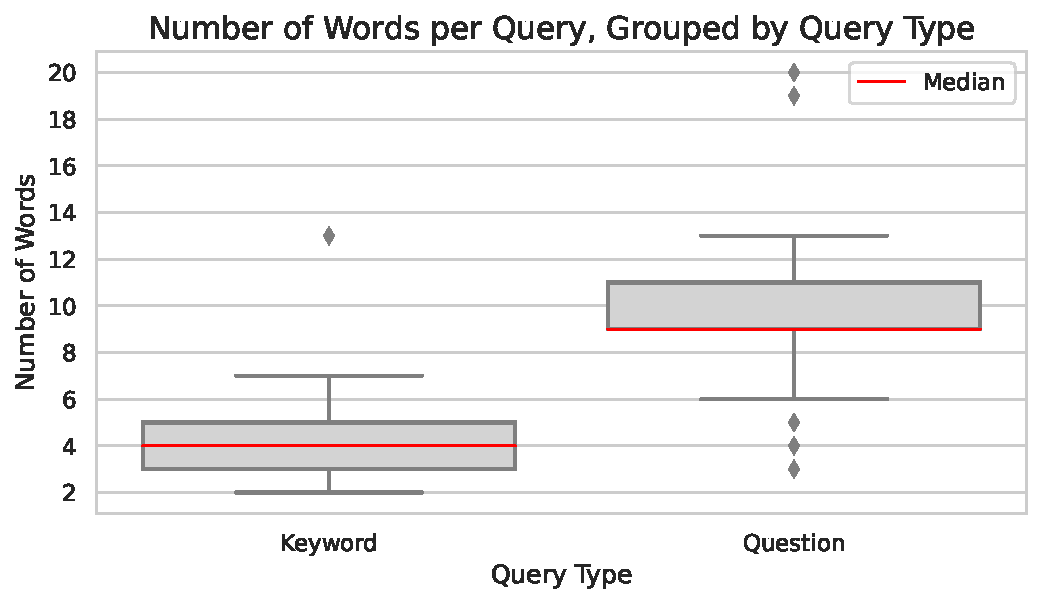
\includegraphics[width=\textwidth]{images/num_words_per_query.pdf}
\caption{Boxplot of the number of words per query, split by query type. Keyword queries are shorter than question queries with a median of 4 words compared to 7 words for the question queries.}
\label{fig:num_words_per_query}
\end{figure}
In total, we identify 17 question-style queries and 33 keyword-style queries by detecting whether the query ends with a question mark.
Figure \ref{fig:num_words_per_query} shows the number of words per query for both query types.
As expected, the keyword queries are shorter than the question queries, with a median of 4 words compared to 7 words for the question queries.
The shortest query is only two words long, while the longest query is 20 words long.
In a later section, we investigate the differences in answer ranking of the different models depending on the two query types.
\subsection{Documents}
\begin{table}
    \centering
    \begin{tabular}{ll}
    \hline
    \textbf{Domain} & \textbf{Occurrences} \\
    \hline
    www.healthline.com & 603 \\
    www.nationalmssociety.org & 419 \\
    www.ms.org.au & 198 \\
    jhu.pure.elsevier.com & 191 \\
    www.msif.org & 183 \\
    www.psychologytoday.com & 161 \\
    www.urotoday.com & 155 \\
    www.news-medical.net & 150 \\
    www.sleepfoundation.org & 141 \\
    www.aafp.org & 139 \\
    \hline
    \end{tabular}
    \captionof{table}{Top 10 Most Frequently Occurring Domains}
    \label{tab:top_domains}
\end{table} 
\begin{figure}
    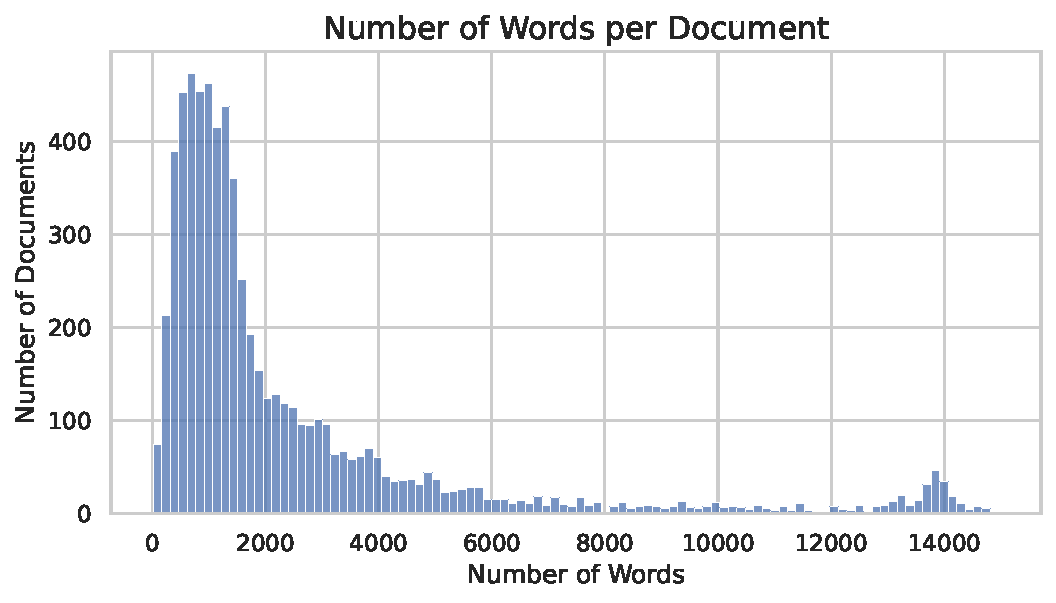
\includegraphics[width=\textwidth]{images/num_words_per_passage.pdf}
    \caption{Histogram of the number of words per document. The plot is cut at 15,000 words, which excludes 120 or 2\% of the documents. The median number of words per document is 1354, while the mean is 2901.}
    \label{fig:num_words_per_document}
\end{figure}
The documents in the dataset are scraped from a total of 234 different web domains.
Table \ref{tab:top_domains} shows the top 10 most frequently occurring domains in the dataset.
Most domains are health-related, belonging to either health organizations, medical journals, or health news websites.
Some domains are more general, e.g. there are also wikipedia.org pages in the dataset, as well as some domains from essay writing or homework help websites.
A total of 133 domains show up less than 10 times in the dataset, while 44 domains show up only once.
After preprocessing, the documents are cleaned of all HTML tags and HTML elements containing fewer than 50 characters.
Figure \ref{fig:num_words_per_document} shows that the number of words per document is high, with a median of 1354 words and a mean of 2901 words.
The high word count is natural for documents scraped from the web, which not only contain the main text but also navigation bars, footers, sidebars, and other elements.
Those can not be fully removed with our heuristic-based preprocessing methods.
\subsection{Document Ratings}
\begin{figure}
\centering
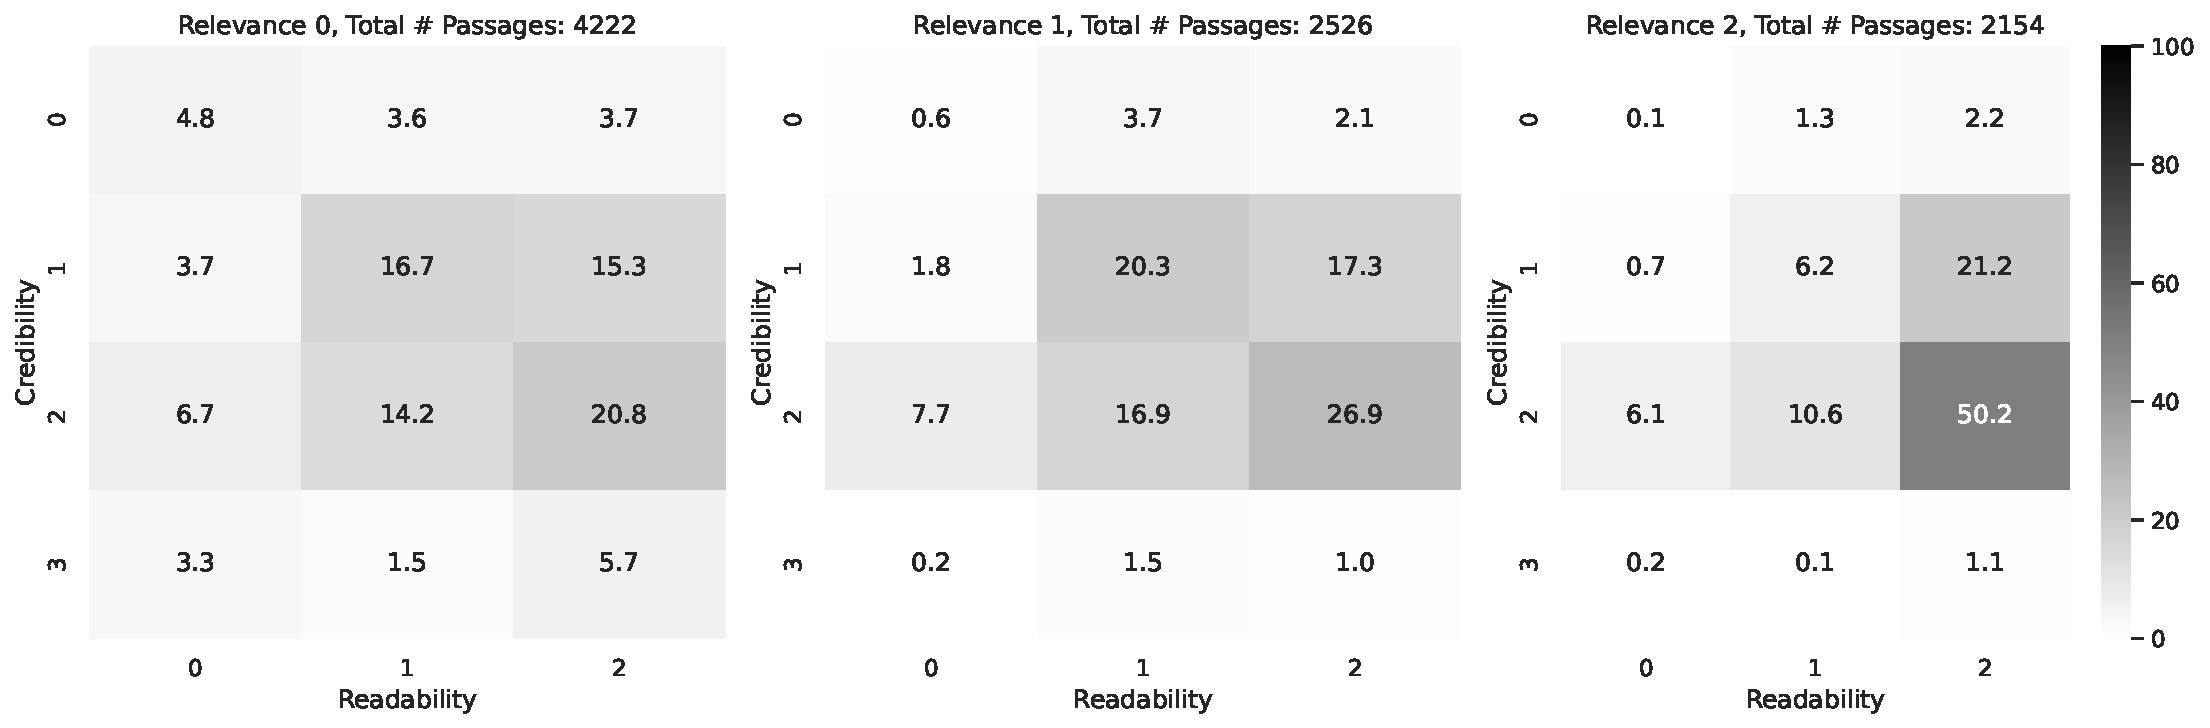
\includegraphics[width=\textwidth]{images/heatmap_qrels.pdf}
\caption{Three heatmaps, one for each relevance score, plotting credibility against readability.
The total number of documents with the given relevance ranking is in the title of the heatmap.
In all three heatmaps, the highest number of documents is concentrated in the range between 1 and 2 for both credibility and readability, with 2 credibility and 2 readability being the most common combination.
}
\label{fig:heatmap_rel_cred_read}
\end{figure}
The evaluation dimensions of readability, credibility, and relevance are the human annotations from the CLEF eHealth 2021 dataset by \cite{goeuriot:2021:Consumer}.
Documents can have multiple ratings for each dimension if they are annotated for multiple queries.
Having multiple annotations for different queries results in the total number of ratings per dimension (8902) being higher than the number of documents in the dataset (6692).

In general, a high number of documents are rated as not relevant to the given query.
Figure \ref{fig:heatmap_rel_cred_read} shows three heatmaps, with each dimension being displayed in a separate heatmap.
Documents rated with 0 relevance make up nearly half of the dataset and generally have lower credibility and readability scores.
The most relevant documents are generally also the most credible and readable ones.
With a value of 0.08, there is no correlation between relevance and credibility.
For readability and relevance, the correlation is 0.22, which is slightly stronger, but still does not show a strong connection.
The correlation scores can be interpreted as the relevance of a document being independent of its credibility and readability, which shows that the annotators were able to judge the relevance of a document independently of its credibility and readability.

\subsection{Documents with Ratings for Multiple Queries}\label{sec:documents-with-multiple-ratings}
As mentioned previously, some documents have multiple ratings for different queries.
In total 875 documents are rated for multiple queries, with the highest number of individual annotations for a single document being 18.
Documents with multiple ratings are often general articles about a certain topic, e.g. ``What is Multiple Sclerosis?''.
Those are then retrieved for multiple queries that focus on different aspects of the topic, e.g. ``List of multiple sclerosis symptoms'' and ``Can I pass multiple sclerosis to other family members?''.
As expected, the different relevance ratings for the same document are often different, since the relevance of a document depends on the query.
Interestingly, we also find that the credibility and readability ratings for the same document can be different.
In Appendix \ref{appendix:dataset}, we show an example of a document with multiple ratings for different queries.
The 15 different ratings cover nearly all possible combinations of relevance, credibility, and readability.

As all documents for one query are annotated by the same person according to \cite{goeuriot:2021:Consumer}, we assume that the annotators were consistent in their ratings for the same query.
Because we are only interested in the ranking of the documents for one query at a time, we do not remove or aggregate the scores, as this could alter the ranking of the documents compared to documents that were only ranked for this specific query.

\section{Retrieval Pipeline Development}
In this section, the implementation of the different retrieval pipelines is discussed.
The baseline models (DPH and TF-IDF), as well as the ColBERT version 1 and the monoT5/duoT5-based pipelines, are implemented in the PyTerrier framework by \cite{pyterrier:2020:Declarative}, which is a Python API for the Terrier IR Platform~(\cite{macdonald:2012:From}).
The ColBERT version 2 pipeline is based on the original implementation provided by the authors.\footnote{\url{https://github.com/stanford-futuredata/ColBERT}, accessed on 04.01.2024}

\subsection{Retrieval Setup}
The retrieval setup in this work differs from the usual retrieval setup, in which a large document collection is indexed, and then multiple queries are run against the index using different retrieval models.
In our case, we build separate indices for each query, containing only the documents that are assessed for that query.
Having separate indices ensures that each document that is retrieved for a query is also assessed for that query.

\subsection{Baseline Models}
This section describes the implementation of the baseline models, namely DPH and TF-IDF.
For both models, the basic indexing function of PyTerrier is used, which indexes and preprocesses the documents.
Preprocessing is done with the default values, which include the following operations:
\begin{itemize}
    \item{\textbf{Tokenization}, for splitting the text into individual words or tokens. The default PyTerrier tokenizer splits text on non-alphanumeric characters. Additional rules to discard tokens that are longer than 20 characters, contain more than 4 digits or contain the same character more than 3 times in a row are applied. All tokens are also converted to lowercase.}
    \item \textbf{Stopword removal}, to remove tokens that do not contain information about the content. We use the default PyTerrier stopword list.
    \item \textbf{Stemming}, to remove the different endings a token can have, leaving only the root of the word. The Porter stemmer, a rule-based stemmer, is used here.
\end{itemize}
The resulting inverted index contains all remaining tokens and a mapping from each token to the documents in which the token occurs.

\begin{figure}[tb]
    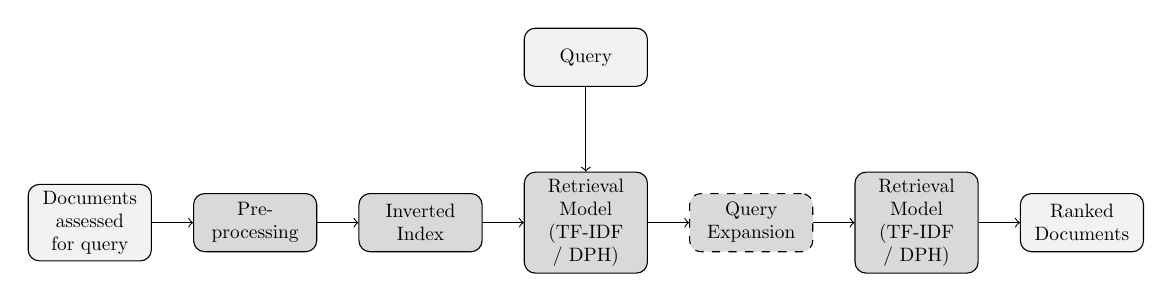
\begin{tikzpicture}[node distance=3cm, every node/.style={scale=0.7}]
    \tikzstyle{box} = [rectangle, draw, fill=gray!10,  text width=2cm, text centered, rounded corners, minimum height=3em]
    \tikzstyle{process} = [rectangle, draw, fill=gray!30,  text width=2cm, text centered, rounded corners, minimum height=3em]
    \node (docCol) [box] {Documents assessed for query};
    \node (preprocess) [process, right of=docCol] {Pre-\\processing};
    \node (invertedindex) [process, right of=preprocess] {Inverted Index};
    \node (retrieval) [process, right of=invertedindex] {Retrieval Model (TF-IDF / DPH)};
    % query expansion with dotted line around
    \node (qe) [process, right of=retrieval, dashed] {Query Expansion};
    \node (reranking) [process, right of=qe] {Retrieval Model (TF-IDF / DPH)};
    \node (ranked) [box, right of=reranking] {Ranked Documents};
    \node (query) [box, above of=retrieval] {Query};

    \draw [->] (docCol) -- (preprocess);
    \draw [->] (preprocess) -- (invertedindex);
    \draw [->] (invertedindex) -- (retrieval);
    \draw [->] (retrieval) -- (qe);
    \draw [->] (qe) -- (reranking);
    \draw [->] (reranking) -- (ranked);
    \draw [->] (query) -- (retrieval);

    \end{tikzpicture}
\caption{Baseline retrieval pipeline, using either TF-IDF or DPH as retrieval model with optional query expansion. This pipeline retrieves and ranks assessed documents for a given query.}
\label{fig:baseline-pipeline}
\end{figure}
The two retrieval models TF-IDF and DPH are then applied using the default parameters, discussed in section \ref{sec:baseline-retrieval-models}.
Both models are tested with and without query expansion.
We use BO1 query expansion, which uses the documents retrieved by the original query to expand the query.
It adds terms from the retrieved documents to the original query based on informativeness, which is a measure of how frequently the term occurs in the documents compared to how frequently the term occurs in the whole collection.
Terms that occur more frequently in the retrieved documents than in the collection are added to the query.
Afterward, the expanded query is run against the index again, and the documents are ranked according to the new query.
The resulting pipeline is shown in Figure \ref{fig:baseline-pipeline}.
The pipeline produces a ranked list of documents for each query, which can then be compared to the order of documents according to the human annotations.

\subsection{Transformer Models}
In addition to the baseline models, we also use the transformer-based models ColBERT version 1 and 2, as well as the monoT5 and duoT5 models.
The implementations of ColBERT version 1 and the monoT5/duoT5 models are done in PyTerrier, while the implementation of ColBERT version 2 is done in the original implementation provided by the authors.

All mentioned models are based on a pre-trained model, which is used to encode the query and the documents in different ways.
Both ColBERT versions are based on the BERT-base model, while the monoT5 and duoT5-based models are based on the T5 model.
The retrieval models themselves are fine-tuned on the MS MARCO passage ranking dataset~(\cite{bajaj:2016:MSMARCO}), a large-scale dataset for passage retrieval.

Transformer-based retrieval models usually require a first retrieval step using a less computationally expensive model like tf-idf, to reduce the number of documents that are fed to the transformer model.
Because in this thesis the retrieval dataset is small, the first retrieval step is omitted for all transformer-based models.

\subsubsection{ColBERT Version 1}
Using the ColBERT implementation for PyTerrier,\footnote{\url{https://github.com/terrierteam/pyterrier_colbert}, accessed on 04.01.2024} an end-to-end pipeline can be constructed from a pre-trained ColBERT model and a document collection.
In our experiments, we use the pre-trained ColBERT checkpoint provided by the authors.
The checkpoint can directly be loaded in the PyTerrier framework, and then used to retrieve documents from the collection.
All parameters are left at their default values.

\subsubsection{monoT5 and duoT5}
Like the ColBERTv1 implementation, the monoT5 and duoT5 implementations are also available in PyTerrier.\footnote{\url{https://github.com/terrierteam/pyterrier_t5}, accessed on 04.01.2024}
Pre-trained checkpoints based on the MS MARCO dataset are provided by the authors.
The monoT5 pipeline generates scores for each query-document pair, which are then used to rank the documents.
The duoT5 pipeline takes the ranking from the monoT5 pipeline and re-ranks the top 10 documents by directly comparing each pair of the top 10 documents directly to the query.
The scores are aggregated to produce a final ranking.
Again, all parameters are left at their default values.

\subsubsection{ColBERT Version 2}
Unlike the other transformer-based models, ColBERT version 2 is not available directly in PyTerrier.
Instead, we use the implementation provided by the authors of the model.\footnote{\url{https://github.com/stanford-futuredata/ColBERT}, accessed on 04.01.2024}
The implementation works with any pre-trained checkpoint for the ColBERT version 2 model, with the MS MARCO checkpoint being downloaded by default.

\subsection{External scores for Readability}\label{sec:external-scores}
To improve retrieval effectiveness for readability, we experiment with adding pre-computed external scores to the retrieval process.
To estimate the readability of the documents in the dataset, different scores are calculated for each document.

The first score is the Flesch Reading Ease (FRE) score devised by \cite{kincaid:1975:Derivation}, which is a score between 0 and 100, with higher scores indicating easier-to-read text.
It is calculated using the following formula, based on average sentence length (ASL) and average number of syllables per word (ASW):
\begin{equation}
    FRE = 206.835 - (1.015 \times ASL) - (84.6 \times ASW)
\end{equation}
We use the implementation provided by the textstat library.\footnote{\url{https://pypi.org/project/textstat/}, accessed on 04.01.2024}
This library also provides the second score, which is an aggregate of multiple similar scores, like the FOG score, the SMOG score, and the Coleman-Liau Index.
Those scores are all based on different text statistics, like the number of syllables per word, the number of words per sentence, or the number of characters per word.
More details about the different scores can be found in the documentation of the textstat library.

\section{Generating LLM Responses}
We now introduce the LLMs that we selected for the experiments, and the steps taken to get the generated answers from the LLMs.
Additionally, the different prompting strategies that are used to generate the responses are described.

\subsection{Selection of Language Models}
We select multiple LLMs for our experiments, which differ in the number of parameters, amount and type of training data, and the type of pre-training and fine-tuning.

\subsubsection{GPT-2}
As a simple baseline and to investigate how an increased number of parameters affects the ranking results, we select different sizes of the GPT-2 model, namely the base, medium, large, and XL versions.
Those models only differ in the number of parameters, which are 124M, 355M, 774M, and 1.5B respectively, while the training objective and the training data are the same for all models.
The dataset used for pre-training is the WebText dataset, which contains 40 GB of web text, which is scraped from URLs shared on Reddit that received at least 3 upvotes.
Other than this pre-training, the models are not fine-tuned to any specific task.

\subsubsection{Models optimized for dialog}\label{sec:dialog-models}
Dialog-optimized models are fine-tuned for the task of interacting with a human in a dialog, usually as a chatbot.
Chatbots are currently the use case of LLMs that comes closest to the task of LFQA, so including models optimized for dialog is a natural choice.
To make a model suitable for directly interacting with humans, different fine-tuning objectives are used in which the behavior of the model is aligned with the expectations of the human.

The importance of this alignment is shown by \cite{ouyang:2022:Training}, who show that answers of their instruction-tuned model InstructGPT are preferred by humans compared to outputs by a model with over 100 times the number of parameters, but without any fine-tuning.
We select the following models:
\begin{description}
\item[Falcon,] which was released in 2023 on HuggingFace.\footnote{\url{https://huggingface.co/blog/falcon}, accessed on 04.01.2024}
At the time of writing, there are three model sizes available, 7B, 40B, and 180B parameters, each as a foundation model or as an instruction-tuned model.
For our experiments, we only use the small 7B instruction-tuned model.

According to the HuggingFace model card, the model is pre-trained on the RefinedWeb dataset by \cite{penedo:2023:The} and then fine-tuned on the GPTeacher,\footnote{\url{https://github.com/teknium1/GPTeacher}, accessed on 04.01.2024} GPT4All\footnote{\url{https://github.com/nomic-ai/gpt4all}, accessed on 04.01.2024} and Baize~(\cite{xu:2023:Baize}) datasets.
GPTeacher and GPT4All are both datasets of prompt-response pairs, while Baize is a dataset based on self-chats by ChatGPT, which have been seeded by questions from Quora, StackOverflow, and MedQuAD.
Unfortunately, the authors do not detail exactly how the data was used to fine-tune the model, as a scientific paper is still yet to be released.


\item[Llama 2,] a model introduced in 2023 by \cite{touvron:2023:Llama}.
It is available through the HuggingFace library, after agreeing to the terms of use posed by Meta.
It comes in three sizes, 7B, 13B, and 70B parameters.
For each of the sizes, the base language model, and a fine-tuned version for chat is available.
In our experiments, we use the fine-tuned version in both the 7B and 13B sizes, since the 70B parameter model is too large to fit on our available hardware.

To create the chat model, the base model is first tuned using supervised fine-tuning, where the model is trained on a dataset of prompt-response pairs, which are all written by humans.
The next step is Reinforcement Learning with Human Feedback (RLHF), by which the model is aligned with human preferences. 
To generate a training set, humans are tasked to evaluate which of two generated responses to a given prompt they prefer.
Based on that data, a reward model is trained, which can then evaluate generated responses on a large scale.
The model is then fine-tuned to maximize the reward given by the reward model.
The RLHF training is done over multiple iterations, continuously improving the reward model and the chat model based on human feedback.
Additionally, they not only optimize for the helpfulness of the generated response but also evaluate for safety, instructing the model not to provide harmful content in that way.


\item[ChatGPT,] is the largest model we used, with 175B parameters. 
It was introduced by OpenAI at the end of 2022.\footnote{\url{https://openai.com/blog/chatgpt/}, accessed on 04.01.2024}
As a commercial product, ChatGPT can only be accessed through the OpenAI API, which we did by using the provided Python library.

With OpenAI becoming more secretive about their models since starting to monetize them, the exact training data and fine-tuning procedure are not known.
In their blog post, they state that the model is a close sibling to the InstructGPT model mentioned above.
Being a sibling model means the fine-tuning procedure is likely similar to the one described by \cite{ouyang:2022:Training} but with a larger model size.
The methods applied are similar to the ones used for the Llama 2 model, first using supervised fine-tuning, and then using RLHF to align the model with human preferences.
\end{description}

Table \ref{tab:language-models} gives an overview of all the used models, comparing parameter size pre-training and fine-tuning data, as well as fine-tuning methods.
In total, we use 8 different models, 4 of which are variants of GPT-2, while the others a different fine-tuned models for chat.
\begin{table}[tb]
\centering
\begin{tabularx}{\textwidth}{lllXXX}
\hline
\textbf{Model} & \textbf{Params} & \textbf{Release} & \textbf{Pre-training Data} & \textbf{Fine-tuneing Data} & \textbf{Fine-tuneing Methods} \\
\hline
GPT-2 Base    & 124M & \multirow{4}{*}{2019} & \multirow{4}{*}{WebText} & \multirow{4}{*}{-} & \multirow{4}{*}{-} \\
GPT-2 Medium  & 355M &                      &                          &  &  \\
GPT-2 Large   & 774M &                      &                          &  &  \\
GPT-2 XL      & 1.5B &                      &                          &  &  \\
\hline
Falcon 7B              & 7B      & 2023 & RefinedWeb           & GPTeacher, GPT4All, Baize & SFT \\
\hline
Llama 2 7B & 7B    & \multirow{2}{*}{2023} & \multirow{2}{*}{Proprietary} & \multirow{2}{*}{Proprietary} & \multirow{2}{*}{SFT, RLHF} \\
Llama 2 13B   & 13B   &  &                        &                         &  \\
\hline
ChatGPT                & 175B   & 2022 & Proprietary                & Proprietary & Proprietary \\
\hline
\end{tabularx}
\caption{Comparison of evaluated Language Models. SFT = Supervised Fine-Tuning, RLHF = Reinforcement Learning with Human Feedback}\label{tab:language-models}
\end{table}

\subsection{Prompting approaches}\label{sec:prompting-approaches}
How a LLM is prompted to complete a task has a large impact on the quality of the generated response.
\cite{reynolds:2021:Prompt} show this impact in the context of translating French to English.
They compare the effect of three different prompting strategies, finding that the most complex one leads to the best translations.
Based on those results we use a similar approach of different prompting strategies for our experiments.
We use the following four strategies:
\begin{enumerate}
    \item \textbf{No Prompt:}\\ \textit{query}
    \item \textbf{Short QA Prompt:}\\ Q: \textit{query}\\A:
    \item \textbf{Long QA Prompt:}\\ Question: \textit{query}\\Answer:
    \item \textbf{MultiMedQA Promp:}\\ You are a helpful medical knowledge assistant. Provide useful, complete, and scientifically grounded answers to common consumer search queries about health.\\Question: \textit{query}\\Complete Answer:
\end{enumerate}
where \textit{query} is replaced by the query to be answered.
Based on the results of \cite{reynolds:2021:Prompt}, we expect the generated answers based on the MultiMedQA prompt to rank highest, followed by the long QA prompt.
To reduce the influence of random variations in the generated responses, we generate 10 responses for each query and model.

\subsection{Generating Answers}
To generate answers for a given query, the query is passed to the LLM using one of the prompting strategies described above.
Most LLMs take additional parameters as input, which are used to guide the text generation process.
The following parameters are considered for the different models in our experiments:
\begin{description}
    \item [Max new tokens] defines the maximum number of new tokens to be generated by the LLM, limiting the length of the generated output.
    \item [Temperature] controls the randomness in the generation process. A higher temperature value increases randomness in the output, while a lower value leads to more deterministic outputs.
    \item [Top k] sets a threshold for the number of most likely next tokens to consider at each step of generation, only allowing the model to choose from the top k tokens. A higher value for k will increase the diversity of the generated output, while a lower value will decrease diversity.
    \item [Top p/nucleus sampling] specifies a cumulative probability threshold. The model will only consider the smallest set of tokens whose cumulative probability does not exceed the threshold.
    \item [Repetition penalty] is used to discourage the model from repeating the same phrases. A repetition penalty greater than 1 will decrease the likelihood of tokens that have already appeared in the generated text, so the model produces more diverse and less repetitive content.
\end{description}
Not all parameters are available for all models and the optimal values for each parameter differ between models.
We chose to set the same values for all models, to make the comparison between the models more consistent.
We did not try to find the optimal values for each model but instead used values we found to work well with all models in manual experiments.
\begin{description}
\item[Maximum number of new tokens] is set to 512 because that's the maximum length of the input for the GPT-2 models.

\item[Temperature] is set to 0.75, restricting the variability of the generated output, while still allowing for some randomness.

\item[Top k and top p] are set to 50 and to 0.95 respectively, which both restrict the number of tokens the model can choose from to more likely tokens.

\item[Repetition penalty] is set to 1.2, which is a relatively low value, but still helps to reduce repetition in the generated output, which we found to be a common problem, especially for the GPT-2 models, but also for the smaller instructing tuned models.
\end{description}
Any additional parameters that are available for a model are left at their default values.

The generating of the answers is done in two different ways.
For ChatGPT, we use the OpenAI API to generate the answers, specifically using the model version ``GPT-3.5-turbo-0613''.
Since they do not provide any parameters apart from temperature and number of tokens, we only set those to our chosen values.

For all other models, we use the HuggingFace library to generate the answers.
The HuggingFace library allows us to set all parameters as described above.
Each model is prompted ten times with each of the prompting strategies, resulting in 40 generated answers per query for each model.